\documentclass[12pt,a4paper,oneside]{report}

% Packages
\usepackage[T1]{fontenc}
\usepackage{lmodern}
\usepackage{geometry}
\usepackage{setspace}
\usepackage{graphicx}
\usepackage{amsmath,amssymb}
\usepackage{booktabs}
\usepackage{tabularx}
\usepackage{array}
\usepackage{float}
\usepackage[font=small,labelfont=bf]{caption}
\usepackage{xcolor}
\usepackage{enumitem}
\usepackage{tikz}
\usetikzlibrary{arrows.meta,positioning,fit,calc}
\usepackage{hyperref}
\usepackage{tocbibind}
\usepackage{titlesec}
\titleformat{\chapter}[hang]{\LARGE\bfseries}{\thechapter.}{0.6em}{}
\titlespacing*{\chapter}{0pt}{-12pt}{14pt}
\setlength{\emergencystretch}{3em}
\setlist{itemsep=1pt, topsep=3pt}

% Page layout
\geometry{left=1.25in, right=1.25in, top=1in, bottom=1in}
\onehalfspacing
\graphicspath{{../figures/}}
\hypersetup{colorlinks=true, linkcolor=black, citecolor=black, urlcolor=blue}
\newcolumntype{Y}{>{\raggedright\arraybackslash}X}

%------------------------------------
% Project details
%------------------------------------
\newcommand{\ProjectTitle}{A Multi-Stage Machine Learning Intrusion Detection Engine for Known and Potentially Novel Network Attacks}
\newcommand{\StudentNames}{Mayank Tiwari (241CV235)\\Narra Shanmukha Srida (241CS238)}
\newcommand{\StudentNamesInline}{Mayank Tiwari (241CV235) and Narra Shanmukha Srida (241CS238)}
\newcommand{\GuideName}{Dr.\ Suresan Pareth}
\newcommand{\Degree}{Minor Degree in Machine Learning}
\newcommand{\Department}{Department of Information Technology}
\newcommand{\College}{National Institute of Technology Karnataka, Surathkal}
\newcommand{\AcademicYear}{2026--2027}
\newcommand{\SubmissionDate}{29/10/2026}
\newcommand{\SubmissionPlace}{NITK Surathkal}

% Every experimental number in this report is generated from the saved
% experiment outputs by make_tables.py (no hand-copied results).
\newcommand{\TotalRows}{2,830,743}
\newcommand{\NumFeatures}{78}
\newcommand{\BenignPct}{80.3}
\newcommand{\DupRows}{256,684}
\newcommand{\DupPct}{9.1}
\newcommand{\InfCount}{4,376}
\newcommand{\EoneTrain}{1,981,516}
\newcommand{\EoneVal}{424,608}
\newcommand{\EoneTest}{424,619}
\newcommand{\EtwoTrainFiles}{Fri PM (PortScan), Fri AM, Mon, Thu PM (Infiltration), Tue, Wed}
\newcommand{\EtwoValFiles}{Thu AM (WebAttacks)}
\newcommand{\EtwoTestFiles}{Fri PM (DDoS)}
\newcommand{\EtwoTestRows}{225,745}
\newcommand{\EoneFusionRecall}{98.27}
\newcommand{\EoneFusionFpr}{4.31}
\newcommand{\EoneFusionPrecision}{84.82}
\newcommand{\EoneFusionAlerts}{43.1}
\newcommand{\EoneGateRecall}{98.03}
\newcommand{\EoneGateFpr}{3.29}
\newcommand{\EoneStackMacroFone}{0.922}
\newcommand{\EoneStackAccuracy}{99.95}
\newcommand{\EoneCascadeMacroFone}{0.614}
\newcommand{\EoneMsPerFlow}{0.075}
\newcommand{\EoneFlowsPerSec}{13,347}
\newcommand{\EoneAeAuc}{0.811}
\newcommand{\EoneAeTpr}{40.5}
\newcommand{\EoneAeFpr}{1.13}
\newcommand{\EtwoGateRecall}{99.94}
\newcommand{\EtwoGateFpr}{96.98}
\newcommand{\EtwoFusionRecall}{100.00}
\newcommand{\EtwoFusionFpr}{97.29}
\newcommand{\EtwoFusionAlerts}{972.9}
\newcommand{\EtwoAeTpr}{51.3}
\newcommand{\EtwoAeFpr}{17.06}
\newcommand{\EtwoUnseen}{DDoS}
\newcommand{\EoneOverlap}{13.8}
\newcommand{\EtwoOverlap}{3.3}
\newcommand{\SvmValFprBefore}{10.8}
\newcommand{\SvmValFprAfter}{3.3}
\newcommand{\SvmSelected}{$D=2048$ random features, $\gamma=0.2$, $\alpha=10^{-6}$, 5 SGD epochs, 500,000 training rows}
\newcommand{\UntunedGateFpr}{10.78}
\newcommand{\UntunedFusionAlerts}{115.9}
\newcommand{\BaselineRows}{100,000}
\newcommand{\EoneRuntime}{4 min 9 s}
\newcommand{\EonePeakMem}{6.5}
\newcommand{\ArchiveShaShort}{c3f26274b36c837c}
\newcommand{\EoneLrRecall}{95.39}
\newcommand{\EoneLrPrecision}{71.16}
\newcommand{\EoneLrFpr}{9.487}
\newcommand{\EoneLrAlerts}{94.9}
\newcommand{\EoneLrAuc}{0.9782}
\newcommand{\EoneRfRecall}{99.69}
\newcommand{\EoneRfPrecision}{99.56}
\newcommand{\EoneRfFpr}{0.109}
\newcommand{\EoneRfAlerts}{1.1}
\newcommand{\EoneRfAuc}{0.9999}
\newcommand{\EoneXgbRecall}{99.83}
\newcommand{\EoneXgbPrecision}{99.65}
\newcommand{\EoneXgbFpr}{0.085}
\newcommand{\EoneXgbAlerts}{0.9}
\newcommand{\EoneXgbAuc}{0.9999}
\newcommand{\EoneGatePrecision}{87.98}
\newcommand{\EoneGateAlerts}{32.9}
\newcommand{\EoneGateAuc}{0.9946}
\newcommand{\EoneRfMacroFone}{0.985}
\newcommand{\EoneXgbMacroFone}{0.961}
\newcommand{\EoneLrMacroFone}{0.869}
\newcommand{\EtwoLrRecall}{99.90}
\newcommand{\EtwoLrPrecision}{86.14}
\newcommand{\EtwoLrFpr}{21.063}
\newcommand{\EtwoLrAlerts}{210.6}
\newcommand{\EtwoLrAuc}{0.9254}
\newcommand{\EtwoRfRecall}{63.50}
\newcommand{\EtwoRfPrecision}{99.79}
\newcommand{\EtwoRfFpr}{0.179}
\newcommand{\EtwoRfAlerts}{1.8}
\newcommand{\EtwoRfAuc}{0.9336}
\newcommand{\EtwoXgbRecall}{62.59}
\newcommand{\EtwoXgbPrecision}{99.84}
\newcommand{\EtwoXgbFpr}{0.132}
\newcommand{\EtwoXgbAlerts}{1.3}
\newcommand{\EtwoXgbAuc}{0.9121}
\newcommand{\EtwoGatePrecision}{57.45}
\newcommand{\EtwoGateAlerts}{969.8}
\newcommand{\EtwoGateAuc}{0.7015}
\newcommand{\EtwoRfMacroFone}{0.000}
\newcommand{\EtwoXgbMacroFone}{0.000}
\newcommand{\EtwoLrMacroFone}{0.000}
\newcommand{\EtwoStackMacroFone}{0.000}
\newcommand{\EtwoAeAuc}{0.751}


\begin{document}

%====================================
% TITLE PAGE
%====================================
\begin{titlepage}
    \centering
    \vspace*{-1.6cm}
    {\Large \textbf{\MakeUppercase{\ProjectTitle}}\par}
    \vfill
    A Project Report submitted in partial fulfilment of the requirements for the award of the degree of\par
    \vspace{0.4cm}
    {\large \textbf{\Degree}\par}
    \vfill
    Submitted by\par
    \vspace{0.3cm}
    {\large \textbf{\StudentNames}\par}
    \vfill
    Under the guidance of\par
    \vspace{0.3cm}
    {\large \textbf{\GuideName}\par}
    \vfill
    
\includegraphics[width=3.2cm]{nitk_logo.png}\par
    \vfill
    {\large \textbf{\Department}\par}
    \vspace{0.2cm}
    {\large \textbf{\College}\par}
    \vspace{0.4cm}
    Academic Year: \AcademicYear\par
\end{titlepage}

\pagenumbering{roman}

\chapter*{Certificate}
\addcontentsline{toc}{chapter}{Certificate}
This is to certify that the project entitled \textbf{``\ProjectTitle''} is a bona fide work carried out by \StudentNamesInline{} under my supervision and guidance in partial fulfilment of the requirements for the award of the degree of \Degree.

\vspace{2cm}
\noindent Project Guide \hfill Head of Department

\vspace{2cm}
\noindent Date: \SubmissionDate \hfill Place: \SubmissionPlace
\clearpage

\chapter*{Declaration}
\addcontentsline{toc}{chapter}{Declaration}
We hereby declare that the project entitled \textbf{``\ProjectTitle''} is our original work carried out under the guidance of \GuideName. This work has not been submitted elsewhere for the award of any degree or diploma, except where acknowledged in the report.

\vspace{2cm}
\noindent Place: \SubmissionPlace \hfill Signature of Students

\noindent Date: \SubmissionDate
\clearpage

\chapter*{Acknowledgement}
\addcontentsline{toc}{chapter}{Acknowledgement}
We express our sincere gratitude to our project guide, \GuideName, for the guidance and feedback provided throughout this work, and to the Head of the Department, the faculty members and the institution for their support and encouragement. We also thank the Canadian Institute for Cybersecurity, University of New Brunswick, for making the CICIDS2017 dataset publicly available.
\clearpage

\chapter*{Abstract}
\addcontentsline{toc}{chapter}{Abstract}
Signature-based intrusion detection recognises only attacks it has rules for, and a single supervised classifier trained on flow records struggles with severe class imbalance, false alarms and unfamiliar traffic. This project designs, implements and evaluates a \textbf{multi-stage machine learning intrusion detection engine} for network flow records. A high-recall approximate RBF support vector machine screens every flow; an out-of-fold stacked ensemble of Random Forest, XGBoost and Logistic Regression names the attack family of screened flows; a benign-only PyTorch autoencoder supplies independent anomaly evidence; and a transparent rule-based fusion step combines the stages while keeping every score. An optional Hidden Markov Model stage for session data is implemented but reported as unavailable, because CICIDS2017 has no session identifiers.

The engine is trained and evaluated on the full CICIDS2017 dataset (\TotalRows{} flows, \NumFeatures{} features, nine traffic families) with preprocessing fitted on training data only, thresholds and hyperparameters selected on validation data, and a single test evaluation. Under a family-stratified split the engine detects \EoneFusionRecall\% of attacks at a \EoneFusionFpr\% benign false-positive rate, attributes attack families with \EoneStackAccuracy\% accuracy, and costs \EoneMsPerFlow{} ms per flow; validation-based tuning reduced the SVM gate's false-positive rate from \SvmValFprBefore\% to \SvmValFprAfter\%. Single tree ensembles nevertheless detect attacks with fewer false alarms than the gate, which is the main bottleneck, while the autoencoder catches rare attacks that the gate misses. A second experiment that holds out entire capture files shows that all models degrade sharply on an unseen attack day, so random-split results on CICIDS2017 overstate real-world performance. The engine is served through a command-line predictor, a FastAPI service and a Streamlit dashboard that share one inference implementation.

\vspace{0.3cm}
\noindent\textbf{Keywords:} Intrusion Detection, CICIDS2017, Support Vector Machine, Stacked Generalisation, Autoencoder, Data Leakage.
\clearpage

\begin{singlespace}
\tableofcontents
\listoffigures
\listoftables
\end{singlespace}
\clearpage
\pagenumbering{arabic}

%====================================
\chapter{Introduction}
%====================================

\section{Background and Motivation}
Networks face continuous denial-of-service floods, credential brute forcing, web exploits, botnets and scans. Classic network intrusion detection systems (NIDS) match traffic against hand-written signatures, which is precise for known attacks but blind to new behaviour and costly to maintain. Machine learning (ML) offers a complementary approach: flow exporters such as CICFlowMeter summarise each connection into dozens of statistical features, supervised models learn to separate benign from malicious flows, and unsupervised models trained only on normal traffic can flag behaviour unlike anything seen before. Published ML results are, however, often inflated by evaluation shortcuts such as random splits of near-duplicate records or thresholds tuned on test data~\cite{arp2022dos,sommer2010outside}. This project builds a detection engine from complementary models and evaluates it with a protocol designed to avoid such shortcuts.

\section{Problem Statement}
Given a CICFlowMeter flow record, the system must decide (i) whether the flow is malicious, (ii) if so, which known attack family it belongs to, and (iii) whether it is anomalous relative to normal traffic even if no known family fits. For every flow the output is a final alert label and severity together with the evidence of every stage. A single supervised classifier covers only (i) and (ii), is sensitive to class imbalance (benign traffic is \BenignPct\% of CICIDS2017) and cannot express that traffic is unfamiliar.

\section{Aim and Objectives}
The aim is to develop and rigorously evaluate a multi-stage ML intrusion detection engine for flow records. The objectives are:
\begin{itemize}
    \item to audit, clean and label CICIDS2017 reproducibly without modifying raw data;
    \item to build leakage-resistant splits and fit all preprocessing on training data only;
    \item to implement a high-recall SVM gate, an out-of-fold stacked family classifier, a benign-only autoencoder and an optional HMM, combined by a transparent fusion policy;
    \item to compare the engine with single-model baselines using recall, false-positive rate, alert volume and latency; and
    \item to serve the engine through a CLI, a REST API and a dashboard sharing one implementation.
\end{itemize}

\section{Scope of the Project}
The system analyses CICFlowMeter flow files offline as a reproducible research prototype for analysts and researchers. Live capture, automatic blocking, online learning and public deployment are out of scope. An anomaly flag means ``unusual relative to benign training traffic'', not proven zero-day detection.

\section{Significance of the Study}
The project shows how complementary detectors can be combined so that each alert stays explainable, quantifies the detection versus false-alarm trade-off that matters to analysts, and measures how strongly the choice of data split changes reported performance on a widely used benchmark.

\section{Research Questions}
\begin{enumerate}[label=\textbf{RQ\arabic*.}, leftmargin=*]
    \item Can an approximate RBF SVM act as a high-recall gate with an acceptable false-positive rate at CICIDS2017 scale?
    \item Does out-of-fold stacking improve attack-family attribution over its base models?
    \item Does a benign-only autoencoder add useful independent evidence?
    \item How does the fused engine compare with single-model baselines?
    \item How much does performance change on a capture file whose attacks were not seen in training?
\end{enumerate}

%====================================
\chapter{Literature Review}
%====================================

\section{Introduction}
This chapter reviews intrusion detection datasets, detection methods, ensembles and evaluation pitfalls to position the design choices of the project.

\section{Existing Approaches}
\textbf{Datasets.} CICIDS2017~\cite{sharafaldin2018toward} captured five days of testbed traffic with scripted benign users and scheduled attacks, and extracted flow features with CICFlowMeter. Ring et al.~\cite{ring2019survey} survey intrusion datasets and their differing realism and labelling quality. Engelen et al.~\cite{engelen2021troubleshooting} and Lanvin et al.~\cite{lanvin2022errors} found flow-construction and labelling errors in CICIDS2017 whose correction changes reported performance.

\textbf{Supervised detection.} Buczak and Guven~\cite{buczak2016survey} survey decision trees, SVMs, ensembles and neural networks for intrusion detection. Random Forest~\cite{breiman2001random} and gradient boosting (XGBoost~\cite{chen2016xgboost}) are strong on tabular flow features. Kernel SVMs~\cite{cortes1995support} scale poorly with data size, which random Fourier features~\cite{rahimi2007random} address by approximating the RBF kernel with an explicit feature map.

\textbf{Ensembles and anomaly detection.} Stacked generalisation~\cite{wolpert1992stacked} trains a meta-learner on base-learner predictions, which must come from data the base learners did not see. Autoencoders trained on normal data use reconstruction error as an anomaly score~\cite{sakurada2014anomaly}; Kitsune~\cite{mirsky2018kitsune} applies an autoencoder ensemble to online intrusion detection. Hidden Markov Models~\cite{rabiner1989tutorial} model sequences of hidden states such as attack stages.

\textbf{Evaluation pitfalls.} Sommer and Paxson~\cite{sommer2010outside} argue that ML intrusion detection is harder than other ML tasks because errors are costly and benign traffic is diverse. Arp et al.~\cite{arp2022dos} catalogue pitfalls such as sampling bias and data snooping, and Kaufman et al.~\cite{kaufman2012leakage} formalise data leakage.

\section{Comparison of Existing Studies}
Table~\ref{tab:litcomp} compares representative works by method and relevance to this project.

\begin{table}[!htbp]
\centering
\caption{Comparison of representative approaches}
\label{tab:litcomp}
\small
\begin{tabularx}{\linewidth}{@{}p{2.6cm}p{3.0cm}Y@{}}
\toprule
\textbf{Work} & \textbf{Method / data} & \textbf{Relevance and limitation} \\
\midrule
Sharafaldin et al.~\cite{sharafaldin2018toward} & CICIDS2017 creation & Benchmark and flow features used here. \\
Engelen et al.~\cite{engelen2021troubleshooting} & Audit of CICIDS2017 & Labelling and flow errors; motivates auditing and cautious claims. \\
Mirsky et al.~\cite{mirsky2018kitsune} & Autoencoder ensemble & Unsupervised and fast, but no attack-family attribution. \\
Wolpert~\cite{wolpert1992stacked} & Stacked generalisation & Combines heterogeneous learners; needs out-of-fold meta-features. \\
Rahimi \& Recht~\cite{rahimi2007random} & Random Fourier features & Scales RBF SVMs to millions of rows; quality depends on feature count. \\
Arp et al.~\cite{arp2022dos} & Pitfalls in security ML & Leakage and sampling bias inflate results; motivates our protocol. \\
\bottomrule
\end{tabularx}
\end{table}

\section{Limitations of Existing Approaches}
Many studies report near-perfect accuracy on CICIDS2017 with a single classifier and a random row split. Because the data contains many exact duplicates and attacks are concentrated in particular capture files, such splits put near-identical flows on both sides and overstate performance. Accuracy is often the headline metric despite extreme imbalance, and single classifiers give no separate evidence for unfamiliar traffic.

\section{Research Gap}
A system is needed that separates screening, attribution and anomaly evidence so that each alert is explainable, is evaluated with leakage-aware splits and operational metrics, and states explicitly when a component (such as temporal modelling) cannot be supported by the data.

\section{Proposed Contribution}
This project contributes a four-stage engine with transparent fusion; a reproducible pipeline with immutable raw data, train-only preprocessing, validation-only tuning, out-of-fold stacking and a single test evaluation; a comparison of a family-stratified split with a capture-file split on the full dataset; and one validated inference engine shared by CLI, REST API and dashboard.

%====================================
\chapter{Dataset and Methodology}
%====================================

\section{Dataset Description}
The project uses the CICIDS2017 \emph{MachineLearningCVE} release~\cite{sharafaldin2018toward,cicids2017web}: eight CSV files covering five working days (two files for Thursday, three for Friday) with \TotalRows{} labelled flows, 78 numeric features and one label column. Table~\ref{tab:files} lists the files and their traffic; Figure~\ref{fig:families} shows the strong imbalance. Benign traffic dominates (\BenignPct\%), while Heartbleed (11 flows) and Infiltration (36) are extremely rare.

\begin{table}[!htbp]
\centering
\caption{CICIDS2017 capture files and their traffic}
\label{tab:files}
\footnotesize
\begin{tabular}{@{}lrrp{6.2cm}@{}}
\toprule
\textbf{File} & \textbf{Flows} & \textbf{Benign} & \textbf{Attack families (flows)} \\
\midrule
Fri PM (DDoS) & 225,745 & 97,718 & DDoS (128,027) \\
Fri PM (PortScan) & 286,467 & 127,537 & PortScan (158,930) \\
Fri AM & 191,033 & 189,067 & Bot (1,966) \\
Mon & 529,918 & 529,918 & none \\
Thu PM (Infiltration) & 288,602 & 288,566 & Infiltration (36) \\
Thu AM (WebAttacks) & 170,366 & 168,186 & WebAttack (2,180) \\
Tue & 445,909 & 432,074 & Patator (13,835) \\
Wed & 692,703 & 440,031 & DoS (252,661), Heartbleed (11) \\
\bottomrule
\end{tabular}
\end{table}


\begin{figure}[!htbp]
\centering
\includegraphics[width=0.66\linewidth]{exp1_row_split/family_distribution.pdf}
\caption{Flows per traffic family in CICIDS2017 (log scale)}
\label{fig:families}
\end{figure}

\section{Feature Description}
Each record summarises one bidirectional flow: volume (packets and bytes per direction), packet-length statistics, timing (duration, inter-arrival, active and idle times), rates (bytes/s, packets/s), TCP flag counts, header and window fields, bulk and subflow statistics, and the destination port. The 15 raw labels are mapped by a versioned file to a binary target and a nine-class family target (BENIGN, Bot, DDoS, DoS, Heartbleed, Infiltration, Patator, PortScan, WebAttack); the raw label is kept for traceability.

\section{Exploratory Data Analysis}
The audit found (i) extreme imbalance spanning five orders of magnitude; (ii) \DupRows{} exact duplicate flows (\DupPct\%); (iii) \InfCount{} infinite values in \texttt{Flow Bytes/s} and \texttt{Flow Packets/s} and further missing values; (iv) eight columns that are zero in every file; (v) strong file structure: each attack family occurs in only one or two capture files and Monday is purely benign (Table~\ref{tab:files}); and (vi) web-attack labels whose dash is corrupted to the Unicode replacement character in the official archive. Finding (v) drives the splitting strategy.

\section{Data Preprocessing}
Raw files are never modified; their SHA-256 checksums and schemas are recorded. Feature columns are coerced to numbers and infinities replaced by missing values, which are imputed with training-split medians; no rows are dropped. Duplicates are flagged rather than deleted so that their effect can be measured. No categorical encoding is needed, and provenance columns (file, row, flow id) are excluded from the features. Features are standardised with statistics from the training split only and stored as 32-bit floats, which halves memory so the full dataset fits on a 16\,GB laptop.

\section{Feature Engineering}
No hand-crafted features are added. The fitted imputer and scaler form a frozen feature contract stored with the deployment manifest, and inference rejects inputs with missing, unexpected or label columns. The HMM uses three emissions (duration, packets/s, mean packet length) when session data exists.

\section{Dataset Splitting}
Two 70/15/15 splits (seed 42) are evaluated:
\begin{enumerate}
    \item \textbf{Experiment 1, family-stratified rows:} rows are assigned at random, stratified on the family label, so every family appears in every partition (\EoneTrain{} / \EoneVal{} / \EoneTest{} flows). This measures closed-set performance but lets near-identical flows fall on both sides.
    \item \textbf{Experiment 2, capture-file split:} whole files are assigned to partitions, reshuffling deterministically until each partition contains benign and attack traffic. Training uses \EtwoTrainFiles; validation \EtwoValFiles; test \EtwoTestFiles{} (\EtwoTestRows{} flows).
\end{enumerate}
Validation data is used for the SVM threshold and hyperparameters and for autoencoder early stopping and thresholding; the test split is used once.

\section{Proposed Methodology}
Figure~\ref{fig:arch} shows the workflow and inference architecture. Each pipeline stage is an independently rerunnable script, and one command runs inspection, cleaning, splitting, preprocessing, training of every stage, fusion-policy export, manifest writing and the frozen test evaluation.

\begin{figure}[!htbp]
\centering
\resizebox{\linewidth}{!}{%
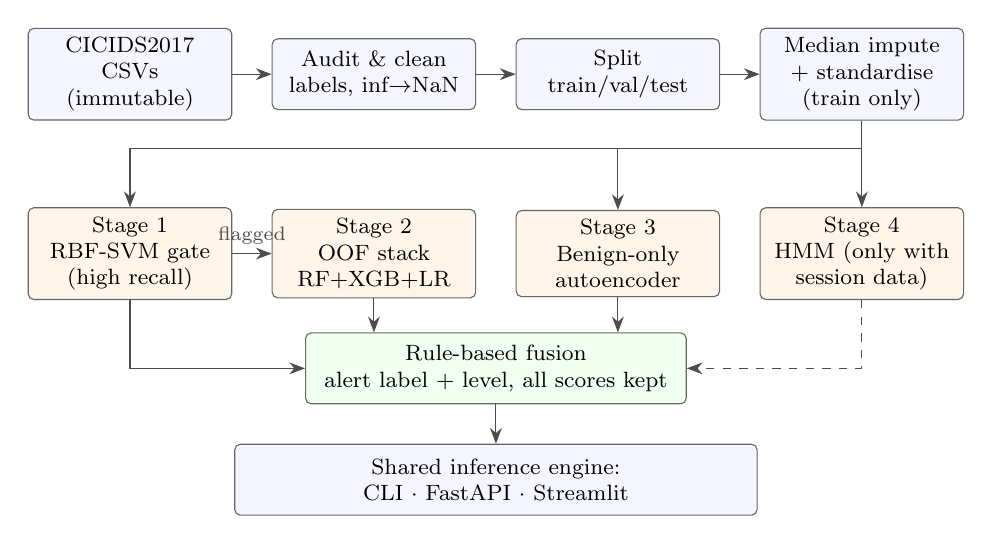
\begin{tikzpicture}[
  node distance=0.45cm and 0.5cm,
  box/.style={draw=black!60, rounded corners=2pt, align=center, font=\footnotesize, minimum height=0.9cm, text width=2.35cm, fill=blue!4},
  stage/.style={box, fill=orange!8},
  arrow/.style={-{Stealth[length=2mm]}, black!70}]
\node[box] (raw) {CICIDS2017 CSVs\\(immutable)};
\node[box, right=of raw] (clean) {Audit \& clean\\labels, inf$\to$NaN};
\node[box, right=of clean] (split) {Split\\train/val/test};
\node[box, right=of split] (prep) {Median impute\\+ standardise\\(train only)};
\node[stage, below=1.1cm of raw] (svm) {Stage 1\\RBF-SVM gate\\(high recall)};
\node[stage, right=of svm] (stack) {Stage 2\\OOF stack\\RF+XGB+LR};
\node[stage, right=of stack] (ae) {Stage 3\\Benign-only\\autoencoder};
\node[stage, right=of ae] (hmm) {Stage 4\\HMM (only with\\session data)};
\node[box, below=1.0cm of $(stack)!0.5!(ae)$, text width=4.6cm, fill=green!6] (fuse) {Rule-based fusion\\alert label + level, all scores kept};
\node[box, below=0.5cm of fuse, text width=6.4cm] (serve) {Shared inference engine: CLI $\cdot$ FastAPI $\cdot$ Streamlit};
\draw[arrow] (raw) -- (clean); \draw[arrow] (clean) -- (split); \draw[arrow] (split) -- (prep);
\draw[arrow] (prep.south) -- ++(0,-0.35) -| (svm.north);
\draw[arrow] (prep.south) -- ++(0,-0.35) -| (ae.north);
\draw[arrow] (prep.south) -- ++(0,-0.35) -| (hmm.north);
\draw[arrow] (svm) -- node[above, font=\scriptsize]{flagged} (stack);
\draw[arrow] (svm.south) |- (fuse.west);
\draw[arrow] (stack.south) -- (stack.south |- fuse.north);
\draw[arrow] (ae.south) -- (ae.south |- fuse.north);
\draw[arrow, dashed] (hmm.south) |- (fuse.east);
\draw[arrow] (fuse) -- (serve);
\end{tikzpicture}}
\caption{Workflow (top) and multi-stage inference architecture (bottom)}
\label{fig:arch}
\end{figure}

\section{Experimental Setup}
\begin{table}[!htbp]
\centering
\caption{Experimental environment}
\label{tab:env}
\small
\begin{tabularx}{\linewidth}{@{}lY@{}}
\toprule
\textbf{Item} & \textbf{Value} \\
\midrule
Hardware & 16-thread laptop CPU, 16\,GB RAM (all models trained on CPU) \\
Software & Python 3.13, scikit-learn, XGBoost, PyTorch 2 (CPU), hmmlearn, pandas, PyArrow, FastAPI, Streamlit \\
Reproducibility & seed 42, versioned YAML configs, SHA-256 data manifest, 30 automated tests \\
Full pipeline run & \EoneRuntime{} for Experiment 1 (peak memory \EonePeakMem\,GB) \\
\bottomrule
\end{tabularx}
\end{table}

%====================================
\chapter{Model Development}
%====================================

\section{Introduction}
The engine has four model stages and a fusion step. Each stage answers a different question, so their errors are partly independent, and each keeps its own score so that analysts can see why an alert was raised.

\section{Algorithm Selection}
\textbf{Stage 1, approximate RBF SVM (binary gate):} a maximum-margin classifier with a non-linear kernel; the kernel is approximated so that training scales to millions of flows, and the threshold is set for high recall so later stages see almost every attack. \textbf{Stage 2, stacked ensemble (family):} Random Forest (bagging), XGBoost (boosting) and Logistic Regression (linear) make different errors, and a Logistic Regression meta-learner combines their probabilities. \textbf{Stage 3, autoencoder (anomaly):} trained on benign flows only, so it needs no attack labels. \textbf{Stage 4, Gaussian HMM (temporal):} models the hidden state of a session when ordered session data exists.

\section{Mathematical Foundations}
\textbf{SVM with random Fourier features.} The RBF kernel $k(\mathbf{x},\mathbf{x}')=\exp(-\gamma\lVert\mathbf{x}-\mathbf{x}'\rVert^2)$ is approximated by $z(\mathbf{x})^\top z(\mathbf{x}')$, where
\begin{equation}
z(\mathbf{x})=\sqrt{2/D}\,\big[\cos(\boldsymbol{\omega}_j^\top\mathbf{x}+b_j)\big]_{j=1}^{D},\qquad \boldsymbol{\omega}_j\sim\mathcal{N}(\mathbf{0},2\gamma I),\; b_j\sim U[0,2\pi]
\end{equation}
for $D$ random features~\cite{rahimi2007random}. A linear SVM on $z(\mathbf{x})$ minimises the class-weighted regularised hinge loss by stochastic gradient descent:
\begin{equation}
\min_{\mathbf{w},b}\; \frac{\alpha}{2}\lVert\mathbf{w}\rVert^2+\frac{1}{n}\sum_{i=1}^{n} c_{y_i}\max\big(0,\,1-y_i(\mathbf{w}^\top z(\mathbf{x}_i)+b)\big),
\end{equation}
with class weights $c_y$ inversely proportional to class frequency. A flow is flagged when $s(\mathbf{x})=\mathbf{w}^\top z(\mathbf{x})+b\ge\tau$, where $\tau$ is the $\lceil 0.98P\rceil$-th largest score among the $P$ validation attacks, the largest threshold giving 98\% validation recall.

\textbf{Out-of-fold stacking.} With $K=5$ stratified folds, each base model $m$ predicts class probabilities $\mathbf{p}_m(\mathbf{x}_i)$ for the fold it was not trained on. The meta-features $\mathbf{q}_i=[\mathbf{p}_{\text{RF}};\mathbf{p}_{\text{XGB}};\mathbf{p}_{\text{LR}}]$ train a multinomial logistic regression $P(y=k\mid\mathbf{q})=\operatorname{softmax}(\mathbf{V}\mathbf{q}+\mathbf{c})_k$; base models are then refitted on all rows. The prediction is $\arg\max_k P(y=k\mid\mathbf{q})$ with confidence $\max_k P(y=k\mid\mathbf{q})$.

\textbf{Autoencoder.} Encoder $f$ and decoder $g$ minimise the mean squared reconstruction error on benign flows. The anomaly score is $a(\mathbf{x})=\frac{1}{d}\lVert\mathbf{x}-g(f(\mathbf{x}))\rVert_2^2$, thresholded at the 99th percentile of benign validation scores (target benign false-positive rate 1\%).

\textbf{HMM.} The forward algorithm gives the filtered state posterior $\boldsymbol{\pi}_t=P(h_t\mid\mathbf{o}_{1:t})$ from past observations only, and the next-state distribution is $\boldsymbol{\pi}_t^\top A$ for transition matrix $A$~\cite{rabiner1989tutorial}.

\textbf{Fusion.} Table~\ref{tab:fusion} lists the rules; the stack is confident when its probability is at least 0.60.

\begin{table}[!htbp]
\centering
\caption{Decision fusion rules}
\label{tab:fusion}
\small
\begin{tabular}{@{}cccll@{}}
\toprule
\textbf{SVM} & \textbf{Conf.\,$\ge$\,0.6} & \textbf{AE} & \textbf{Final label} & \textbf{Level} \\
\midrule
yes & yes & yes & known\_attack\_suspected & high \\
yes & yes & no & known\_attack\_suspected & medium \\
no & -- & yes & anomaly\_review & medium \\
yes & no & any & suspicious\_unclassified & low \\
no & -- & no & benign & none \\
\bottomrule
\end{tabular}
\end{table}

\section{Model Architecture or Algorithm Steps}
The autoencoder maps 78 inputs through layers of 128, 64 and 16 (bottleneck) units and back through 64 and 128 to 78 outputs, with ReLU hidden activations and a linear output. For a batch of flows, inference (i) validates the schema, rejecting label, unknown and duplicate columns and infinities, then imputes and standardises; (ii) scores every flow with the SVM gate; (iii) runs the stack only on gated flows; (iv) scores every flow with the autoencoder; (v) adds HMM context when session identifiers exist; and (vi) applies the fusion rules, returning every stage's output and the model version.

\section{Model Training}
All models use the 78 standardised features. The SVM gate is trained on a class-stratified sample of the training split with balanced class weights, and its threshold is selected on the validation split. The stack is trained on attack rows only (at most 100,000, sampled per family so that every family keeps at least two rows) with the family target. The autoencoder is trained on up to 100,000 benign flows with Adam (learning rate $10^{-3}$, batch 256) for at most 100 epochs, with early stopping (patience 10) on up to 50,000 benign validation flows.

\section{Hyperparameter Selection}
The SVM gate was tuned by grid search on the validation split only, minimising the benign false-positive rate at the threshold that gives 98\% validation recall. Round~1 varied the number of random features, $\alpha$ and the number of epochs; round~2 added the kernel width $\gamma$ and the training-sample size (Table~\ref{tab:svmtuning}). The original setting (one SGD pass, $\alpha=10^{-4}$, $D=512$, 100k rows) gave a validation false-positive rate of \SvmValFprBefore\%; the selected setting gives \SvmValFprAfter\%. Other models use common defaults (Table~\ref{tab:hyper}).

\begin{table}[!htbp]
\centering
\caption{SVM gate hyperparameter search on the validation split (first row: original setting; bold: selected)}
\label{tab:svmtuning}
\small
\begin{tabular}{@{}rrrrrrrr@{}}
\toprule
\textbf{$D$} & \textbf{$\alpha$} & \textbf{Epochs} & \textbf{$\gamma$} & \textbf{Rows} & \textbf{Val.\ FPR (\%)} & \textbf{Val.\ AUC} & \textbf{Fit (s)} \\
\midrule
512 & $10^{-4}$ & 1 & scale & 100k & 10.79 & 0.9873 & 0.3 \\
\textbf{2048} & $10^{-6}$ & \textbf{5} & \textbf{0.2} & \textbf{500k} & \textbf{3.29} & \textbf{0.9945} & \textbf{19.9} \\
2048 & $10^{-6}$ & 5 & 0.05 & 500k & 3.41 & 0.9948 & 28.3 \\
2048 & $10^{-5}$ & 5 & 0.2 & 500k & 3.72 & 0.9932 & 20.2 \\
512 & $10^{-6}$ & 5 & scale & 500k & 3.95 & 0.9920 & 5.1 \\
2048 & $10^{-5}$ & 5 & 0.05 & 500k & 3.98 & 0.9915 & 20.0 \\
512 & $10^{-6}$ & 5 & 0.05 & 500k & 4.08 & 0.9930 & 5.0 \\
\bottomrule
\end{tabular}
\par\smallskip\parbox{\linewidth}{\footnotesize FPR measured at the threshold giving 98\% validation recall. 36 configurations were evaluated in two rounds; the six best of round 2 are shown.}
\end{table}


\begin{table}[!htbp]
\centering
\caption{Final hyperparameters}
\label{tab:hyper}
\small
\begin{tabularx}{\linewidth}{@{}lY@{}}
\toprule
\textbf{Model} & \textbf{Setting} \\
\midrule
SVM gate & \SvmSelected; balanced class weights; recall target 0.98 \\
Random Forest & 200 trees, balanced class weights \\
XGBoost & 200 trees, depth 6, learning rate 0.08, subsample and column sample 0.9 \\
Logistic Regression & base and meta learner, balanced class weights \\
Stacking & 5 stratified folds, $\le$100k rows, confidence threshold 0.60 \\
Autoencoder & 128-64-16, Adam $10^{-3}$, batch 256, $\le$100 epochs, patience 10 \\
HMM & Gaussian, diagonal covariance, 2 states, 3 emission features \\
\bottomrule
\end{tabularx}
\end{table}

\section{Implementation Details}
The system is a Python package (\texttt{src/ids}) plus numbered pipeline scripts. A single \texttt{InferenceEngine} is shared by the CLI predictor, the FastAPI service (\texttt{/health}, \texttt{/model-info}, \texttt{/predict}, \texttt{/predict-batch}, \texttt{/predict-file}; at most 10,000 rows or 10\,MB per request) and the Streamlit dashboard. Training writes a versioned manifest of features, labels and thresholds, and loading fails if the saved models disagree with it.

%====================================
\chapter{Results and Discussion}\label{chap:results}
%====================================

\section{Introduction}
Both experiments use identical models and hyperparameters and differ only in the split. Experiment~1 is the main closed-set evaluation; Experiment~2 tests generalisation to an unseen capture file. Baselines (Logistic Regression, Random Forest, XGBoost) are trained on the same budget as the SVM gate's original setting (\BaselineRows{} family-stratified rows) with a 0.5 probability threshold. All results are on test data.

\section{Evaluation Metrics}
With attacks as the positive class: recall (detection rate) $=\frac{TP}{TP+FN}$; precision $=\frac{TP}{TP+FP}$; $F_1=\frac{2PR}{P+R}$; false-positive rate (FPR) $=\frac{FP}{FP+TN}$, also given as alerts per 1000 benign flows (analyst workload); ROC-AUC summarises ranking quality. Family attribution uses macro-F1, so that rare families count equally. Accuracy is not a headline metric: labelling everything benign would score \BenignPct\%. Latency is the complete engine's time per flow.

\section{Experimental Results}
Table~\ref{tab:binary} and Figure~\ref{fig:rocpr} compare binary detection in Experiment~1.

\begin{table}[!htbp]
\centering
\caption{Binary detection on the Experiment 1 test set (attack = positive class)}
\label{tab:binary}
\small
\resizebox{\linewidth}{!}{\begin{tabular}{@{}lrrrrrrr@{}}
\toprule
\textbf{Model} & \textbf{Prec.\,\%} & \textbf{Rec.\,\%} & \textbf{F1\,\%} & \textbf{FPR\,\%} & \textbf{Alerts/1k} & \textbf{ROC-AUC} & \textbf{ms/flow} \\
\midrule
Logistic regression & 71.16 & 95.39 & 81.51 & 9.487 & 94.9 & 0.9782 & 0.0001 \\
Random forest & 99.56 & 99.69 & 99.62 & 0.109 & 1.1 & 0.9999 & 0.0007 \\
XGBoost & 99.65 & 99.83 & 99.74 & 0.085 & 0.9 & 0.9999 & 0.0002 \\
SVM gate (validation-tuned) & 87.98 & 98.03 & 92.73 & 3.285 & 32.9 & 0.9946 & 0.0066 \\
Full fused system & 84.82 & 98.27 & 91.05 & 4.314 & 43.1 & -- & 0.0749 \\
\bottomrule
\end{tabular}}
\par\smallskip\parbox{\linewidth}{\footnotesize Baselines use a 0.5 probability threshold; the SVM gate uses its validation-tuned threshold. ms/flow for baselines and the gate is model scoring only; for the fused system it is the complete engine including validation and fusion.}
\end{table}


\begin{figure}[!htbp]
\centering
\includegraphics[width=0.84\linewidth]{exp1_row_split/roc_pr_binary.pdf}
\caption{ROC (log-scaled FPR) and precision-recall curves, Experiment~1 test set}
\label{fig:rocpr}
\end{figure}

The fused engine detects \EoneFusionRecall\% of attacks with \EoneFusionAlerts{} alerts per 1000 benign flows at \EoneMsPerFlow{} ms per flow (about \EoneFlowsPerSec{} flows/s in one CPU process). Table~\ref{tab:multiclass} compares family attribution on true attack flows, and Table~\ref{tab:perclass} gives per-family results of the stack.

\begin{table}[!htbp]
\centering
\caption{Attack-family attribution on true attack flows of the Experiment 1 test set}
\label{tab:multiclass}
\small
\resizebox{\linewidth}{!}{\begin{tabular}{@{}lrrrr@{}}
\toprule
\textbf{Model} & \textbf{Accuracy\,\%} & \textbf{Macro-F1} & \textbf{Weighted-F1} & \textbf{Bal.\ acc.\,\%} \\
\midrule
Random forest & 99.96 & 0.985 & 1.000 & 97.60 \\
XGBoost & 99.97 & 0.961 & 1.000 & 93.47 \\
Logistic regression & 99.57 & 0.869 & 0.996 & 90.52 \\
Stacked ensemble (OOF meta) & 99.95 & 0.922 & 0.999 & 97.70 \\
\bottomrule
\end{tabular}}
\par\smallskip\parbox{\linewidth}{\footnotesize Base models are the stack's own base learners refitted on its 8-family training sample. The end-to-end cascade (gate misses counted as errors) has macro-F1 0.614.}
\end{table}


\begin{table}[!htbp]
\centering
\caption{Per-family results of the stacked ensemble (Experiment 1 test set)}
\label{tab:perclass}
\small
\begin{tabular}{@{}lrrrr@{}}
\toprule
\textbf{Family} & \textbf{Precision\,\%} & \textbf{Recall\,\%} & \textbf{F1\,\%} & \textbf{Test flows} \\
\midrule
DoS & 99.97 & 99.95 & 99.96 & 37,900 \\
PortScan & 99.99 & 99.93 & 99.96 & 23,840 \\
DDoS & 99.99 & 99.98 & 99.98 & 19,205 \\
Patator & 100.00 & 100.00 & 100.00 & 2,076 \\
WebAttack & 94.44 & 98.78 & 96.56 & 327 \\
Bot & 100.00 & 99.66 & 99.83 & 296 \\
Infiltration & 27.78 & 83.33 & 41.67 & 6 \\
Heartbleed & 100.00 & 100.00 & 100.00 & 3 \\
\bottomrule
\end{tabular}
\end{table}


The autoencoder, trained without attack labels, reaches a ROC-AUC of \EoneAeAuc{} and flags \EoneAeTpr\% of attacks at a \EoneAeFpr\% benign false-positive rate (target 1\%). Figures~\ref{fig:ae} and~\ref{fig:detection} show its score separation and which families each detector catches.

\begin{figure}[!htbp]
\centering
\includegraphics[width=0.68\linewidth]{exp1_row_split/autoencoder_scores.pdf}
\caption{Autoencoder reconstruction error for benign and attack test flows (Experiment~1)}
\label{fig:ae}
\end{figure}

\begin{figure}[!htbp]
\centering
\includegraphics[width=0.68\linewidth]{exp1_row_split/detection_by_family.pdf}
\caption{Fraction of test flows flagged per attack family by the SVM gate and the autoencoder}
\label{fig:detection}
\end{figure}

\section{Confusion Matrix}
Figure~\ref{fig:confusion} shows the stack's row-normalised confusion matrix on attack flows and Figure~\ref{fig:alerts} the engine's final alert labels per true family.

\begin{figure}[!htbp]
\centering
\begin{minipage}[t]{0.47\linewidth}
\centering
\includegraphics[width=\linewidth]{exp1_row_split/stack_confusion.pdf}
\caption{Stacked ensemble confusion matrix on attack flows (row-normalised)}
\label{fig:confusion}
\end{minipage}\hfill
\begin{minipage}[t]{0.51\linewidth}
\centering
\includegraphics[width=\linewidth]{exp1_row_split/alert_breakdown.pdf}
\caption{Final alert label by true family (row-normalised; $\le$20,000 test flows per family)}
\label{fig:alerts}
\end{minipage}
\end{figure}

Given a true attack flow, the stacked ensemble assigns the correct family to \EoneStackAccuracy\% of flows (Figure~\ref{fig:confusion}, Table~\ref{tab:perclass}). Every family except Infiltration is recognised with recall of at least 98.8\%. The weak point is Infiltration, with only six test flows. Five of the six are identified correctly (recall 83\%), but 13 flows from other families are also labelled Infiltration, so its precision is only 28\% and its F1 is 0.42. The balanced class weights give this 36-flow class a very large weight, which pushes borderline flows towards it.

Figure~\ref{fig:alerts} shows the end-to-end picture. Flows from the large families are almost all labelled \texttt{known\_attack\_suspected}. Most Heartbleed and Infiltration flows receive \texttt{anomaly\_review}: the SVM gate misses them, but the autoencoder flags them as unusual. Most WebAttack flows end as \texttt{benign}, because both the gate and the autoencoder miss them.


\section{Comparison of Models}
\textbf{Binary detection.} On the Experiment~1 test set the single tree ensembles are the strongest binary detectors (Table~\ref{tab:binary}): XGBoost reaches \EoneXgbRecall\% recall at \EoneXgbFpr\% FPR (\EoneXgbAlerts{} alerts per 1000 benign flows), and Random Forest \EoneRfRecall\% at \EoneRfFpr\%. The tuned SVM gate reaches its designed recall (\EoneGateRecall\%) but at a higher false-positive rate (\EoneGateFpr\%, ROC-AUC \EoneGateAuc), and Logistic Regression is the weakest (\EoneLrFpr\% FPR). The fused system inherits the gate's recall and adds the autoencoder's anomaly alerts, giving \EoneFusionRecall\% recall at \EoneFusionFpr\% FPR. The multi-stage design therefore does not beat a well-configured tree ensemble on raw binary accuracy in this closed-set setting. Its value is in attribution, independent anomaly evidence and explainability, and its binary performance is limited by the gate.

\textbf{Family attribution.} All four models attribute families of true attack flows with more than 99.5\% accuracy (Table~\ref{tab:multiclass}). On macro-F1, which weights the six-flow Infiltration class equally with DoS, the Random Forest base learner (\EoneRfMacroFone) scores higher than the stacked ensemble (\EoneStackMacroFone), XGBoost (\EoneXgbMacroFone) and Logistic Regression (\EoneLrMacroFone). Stacking therefore did not improve over its best base model here. Its meta-learner is trained with balanced class weights on out-of-fold probabilities, and with only a few dozen Infiltration and Heartbleed rows the meta-learner's estimates for these classes are noisy.

\textbf{Generalisation to an unseen capture.} In Experiment~2 the test file is the Friday afternoon DDoS capture, and DDoS never appears in training. The trained models behave very differently there (Table~\ref{tab:experiments}). The tree ensembles keep their precision but detect only \EtwoRfRecall\% (Random Forest) and \EtwoXgbRecall\% (XGBoost) of the unseen DDoS flows. The SVM gate's threshold was calibrated on the only validation file, which contains web attacks. On the new day it flags almost all traffic: \EtwoGateRecall\% of attacks but also \EtwoGateFpr\% of benign flows. The autoencoder's benign false-positive rate rises from \EoneAeFpr\% to \EtwoAeFpr\%, which shows that benign traffic itself shifts between capture days. When the family classifier is given true DDoS flows, it labels them as the closest known families: about 84\% as DoS and 16\% as PortScan (from the Experiment~2 confusion matrix).



\begin{table}[!htbp]
\centering
\caption{Experiment 1 (family-stratified rows) vs.\ Experiment 2 (capture-file split)}
\label{tab:experiments}
\small
\begin{tabular}{@{}p{4.8cm}p{3.6cm}p{3.6cm}@{}}
\toprule
\textbf{Metric} & \textbf{Experiment 1} & \textbf{Experiment 2} \\
\midrule
Test flows & 424,619 & 225,745 \\
Attack families in test & Bot, DDoS, DoS, Heartbleed, Infiltration, Patator, PortScan, WebAttack & DDoS \\
Families unseen in training & none & DDoS \\
Test flows with exact copy in train & 13.8\% & 3.3\% \\
SVM gate recall / FPR & 98.03 / 3.29 & 99.94 / 96.98 \\
Autoencoder attack TPR / benign FPR & 40.46 / 1.13 & 51.32 / 17.06 \\
Fused recall / FPR & 98.27 / 4.31 & 100.00 / 97.29 \\
Fused alerts per 1000 benign & 43.1 & 972.9 \\
Stack accuracy on attack flows & 99.95\% & 0.00\% \\
\bottomrule
\end{tabular}
\end{table}


\section{Interpretation of Results}
\textbf{Why tree ensembles dominate.} CICFlowMeter features have heterogeneous scales and heavy tails, and many attacks are separated by sharp thresholds on a few features (destination port, initial window size, header lengths and packet-length maxima; Table~\ref{tab:features}). Axis-aligned tree splits capture such rules directly. The approximate RBF SVM must express the same boundaries through a smooth kernel on standardised features, using 2048 random features and a 500k-row sample. Validation-based tuning cut its false-positive rate from \SvmValFprBefore\% to \SvmValFprAfter\%, but it remains well behind the trees.

\textbf{Why the split matters so much.} \DupPct\% of all flows are exact duplicates. Under the family-stratified split, \EoneOverlap\% of test flows have an identical feature vector in the training set, compared with \EtwoOverlap\% under the capture-file split. Closed-set results are therefore partly a measure of recognition, not generalisation. The large drop in Experiment~2 matches the ``closed world'' concern of Sommer and Paxson~\cite{sommer2010outside}: models learn the attacks and the benign traffic of the days they saw.

\textbf{Value of the anomaly stage.} The autoencoder alone is a weak detector (ROC-AUC \EoneAeAuc, \EoneAeTpr\% of attacks flagged at \EoneAeFpr\% benign FPR), but it is complementary. It flags exactly the rare families the gate misses, and these become \texttt{anomaly\_review} alerts instead of silent misses. The anomaly stage contributes coverage of unusual traffic, not overall accuracy.

\textbf{Feature importance and shortcuts.} The destination port is the single most important Random Forest feature. In CICIDS2017 several attacks target fixed ports (for example FTP and SSH brute forcing, and web attacks on port 80), so this feature can act as a dataset-specific shortcut that would not transfer to networks with different services.


\section{Error Analysis}
\begin{itemize}
    \item \textbf{Web attacks are mostly missed.} Only about 10\% of WebAttack test flows pass the SVM gate, and the autoencoder flags few of them, so most are labelled benign (Figure~\ref{fig:detection}). Brute-force and XSS requests are ordinary-looking HTTP flows to port 80 whose statistics overlap heavily with benign web browsing. The family classifier separates them well once they are gated (F1 above 96\%), so the gate is the bottleneck.
    \item \textbf{Bot traffic is partly missed.} About 59\% of Bot flows are detected; the missed ones are likely low-volume periodic connections whose statistics resemble benign traffic.
    \item \textbf{Rare families rely on the anomaly stage.} The gate detects only one of three Heartbleed flows and one of six Infiltration flows, but the autoencoder flags most of them. With so few examples, per-family estimates for these classes have very high variance.
    \item \textbf{False positives.} \EoneFusionAlerts{} of every 1000 benign flows raise an alert. Most come from the gate (\EoneGateAlerts{} per 1000) and the rest from anomaly alerts on unusual but benign flows (the autoencoder's \EoneAeFpr\% design rate).
    \item \textbf{Cascade metric.} When gate misses are counted as a separate wrong class, the end-to-end family macro-F1 is \EoneCascadeMacroFone. This value is driven mainly by the missed WebAttack, Bot and rare-family flows above, not by attribution errors.
\end{itemize}


\section{Limitations}
CICIDS2017 is a testbed capture with known labelling errors~\cite{engelen2021troubleshooting,lanvin2022errors}, and Heartbleed and Infiltration are too rare for reliable per-family estimates. Closed-set results include near-duplicates across partitions. The SVM gate is an approximation trained on a 500k-row sample, and the stack and autoencoder use 100k-row samples. The destination port may act as a shortcut feature, the HMM could not be evaluated without session identifiers, and the fusion thresholds are fixed rules rather than optimised values.

%====================================
\chapter{Conclusion and Future Work}
%====================================

\section{Summary of the Project}
A reproducible multi-stage intrusion detection engine was built for network flow records and evaluated on the full CICIDS2017 dataset. Raw data is audited without modification, preprocessing is fitted on training data, thresholds and hyperparameters are selected on validation data, and test data is used once. An approximate RBF SVM gate, an out-of-fold stacked family classifier, a benign-only autoencoder and an optional HMM are combined through transparent fusion and served by a CLI, a REST API and a dashboard sharing one inference implementation.

\section{Achievement of Objectives}
All objectives were met: the dataset was audited (duplicates, non-finite values, constant columns, corrupted labels) and labelled reproducibly; two leakage-aware splits were implemented; all stages and the fusion step were implemented and covered by 30 automated tests; the engine was compared with baselines on recall, false-positive rate, alert volume and latency; and the CLI and API outputs were verified to agree.

\section{Major Findings}
\begin{enumerate}
    \item \textbf{Gate (RQ1):} an approximate RBF SVM can serve as a 98\%-recall gate at full CICIDS2017 scale. Its false-positive rate depends strongly on hyperparameters: validation-based tuning reduced it from \SvmValFprBefore\% to \SvmValFprAfter\% (test: \EoneGateFpr\%). It remains the main source of false alarms and missed web attacks.
    \item \textbf{Stacking (RQ2):} family attribution is above 99.5\% accurate for all models, but out-of-fold stacking did not improve macro-F1 over its best base learner, the Random Forest (\EoneStackMacroFone{} vs.\ \EoneRfMacroFone), because of very rare families.
    \item \textbf{Autoencoder (RQ3):} the benign-only autoencoder is weak alone but complementary. It turns most rare-family flows missed by the gate (Heartbleed, Infiltration) into \texttt{anomaly\_review} alerts.
    \item \textbf{Baselines (RQ4):} single tree ensembles (XGBoost: \EoneXgbRecall\% recall at \EoneXgbFpr\% FPR) beat the fused engine on binary detection in the closed-set setting. The engine's advantages are explainable, staged evidence and family attribution, at \EoneMsPerFlow{} ms per flow.
    \item \textbf{Generalisation (RQ5):} on an unseen capture day with an unseen attack family, every model degrades. Tree ensembles miss over a third of the DDoS flows, the gate's validation-calibrated threshold flags most benign traffic, and benign traffic itself shifts. Results from random splits of CICIDS2017 (where \EoneOverlap\% of test flows have an exact copy in training) substantially overstate real-world performance.
\end{enumerate}


\section{Limitations}
The main limitations are the testbed nature and label errors of CICIDS2017, the dependence of results on the split, bounded training samples, the possible destination-port shortcut and the lack of session data for the temporal stage.

\section{Future Work}
\begin{itemize}
    \item Replace or complement the SVM gate with a tree-based gate, and tune the fusion thresholds on validation data against an explicit alert budget.
    \item Evaluate on the corrected CICIDS2017 release~\cite{engelen2021troubleshooting} and other datasets, and run withheld-family experiments for every family.
    \item Replace the destination port with protocol-level features, reconstruct sessions so the HMM can be evaluated, and connect a live CICFlowMeter feed to the API.
\end{itemize}

%====================================
% REFERENCES
%====================================
\begin{singlespace}
\begin{thebibliography}{99}
\small
\setlength{\itemsep}{2pt}
\bibitem{sharafaldin2018toward} I.~Sharafaldin, A.~H. Lashkari and A.~A. Ghorbani, ``Toward generating a new intrusion detection dataset and intrusion traffic characterization,'' in \textit{Proc.\ 4th Int.\ Conf.\ Information Systems Security and Privacy (ICISSP)}, 2018, pp.~108--116.
\bibitem{cicids2017web} Canadian Institute for Cybersecurity, ``Intrusion Detection Evaluation Dataset (CIC-IDS2017),'' University of New Brunswick. URL: \url{https://www.unb.ca/cic/datasets/ids-2017.html}, Accessed: 28 October 2026.
\bibitem{engelen2021troubleshooting} G.~Engelen, V.~Rimmer and W.~Joosen, ``Troubleshooting an intrusion detection dataset: the CICIDS2017 case study,'' in \textit{Proc.\ IEEE Security and Privacy Workshops (SPW)}, 2021, pp.~7--12.
\bibitem{lanvin2022errors} M.~Lanvin, P.-F. Gimenez, Y.~Han, F.~Majorczyk, L.~M\'e and E.~Totel, ``Errors in the CICIDS2017 dataset and the significant differences in detection performances it makes,'' in \textit{Proc.\ 17th Int.\ Conf.\ Risks and Security of Internet and Systems (CRiSIS)}, LNCS, Springer, 2022, pp.~18--33.
\bibitem{ring2019survey} M.~Ring, S.~Wunderlich, D.~Scheuring, D.~Landes and A.~Hotho, ``A survey of network-based intrusion detection data sets,'' \textit{Computers \& Security}, vol.~86, pp.~147--167, 2019.
\bibitem{buczak2016survey} A.~L. Buczak and E.~Guven, ``A survey of data mining and machine learning methods for cyber security intrusion detection,'' \textit{IEEE Communications Surveys \& Tutorials}, vol.~18, no.~2, pp.~1153--1176, 2016.
\bibitem{sommer2010outside} R.~Sommer and V.~Paxson, ``Outside the closed world: On using machine learning for network intrusion detection,'' in \textit{Proc.\ IEEE Symp.\ Security and Privacy}, 2010, pp.~305--316.
\bibitem{arp2022dos} D.~Arp \textit{et al.}, ``Dos and don'ts of machine learning in computer security,'' in \textit{Proc.\ 31st USENIX Security Symposium}, 2022.
\bibitem{kaufman2012leakage} S.~Kaufman, S.~Rosset, C.~Perlich and O.~Stitelman, ``Leakage in data mining: Formulation, detection, and avoidance,'' \textit{ACM Trans.\ Knowledge Discovery from Data}, vol.~6, no.~4, 2012.
\bibitem{cortes1995support} C.~Cortes and V.~Vapnik, ``Support-vector networks,'' \textit{Machine Learning}, vol.~20, no.~3, pp.~273--297, 1995.
\bibitem{rahimi2007random} A.~Rahimi and B.~Recht, ``Random features for large-scale kernel machines,'' in \textit{Advances in Neural Information Processing Systems (NIPS)}, 2007.
\bibitem{breiman2001random} L.~Breiman, ``Random forests,'' \textit{Machine Learning}, vol.~45, no.~1, pp.~5--32, 2001.
\bibitem{chen2016xgboost} T.~Chen and C.~Guestrin, ``XGBoost: A scalable tree boosting system,'' in \textit{Proc.\ 22nd ACM SIGKDD Int.\ Conf.\ Knowledge Discovery and Data Mining}, 2016, pp.~785--794.
\bibitem{wolpert1992stacked} D.~H. Wolpert, ``Stacked generalization,'' \textit{Neural Networks}, vol.~5, no.~2, pp.~241--259, 1992.
\bibitem{sakurada2014anomaly} M.~Sakurada and T.~Yairi, ``Anomaly detection using autoencoders with nonlinear dimensionality reduction,'' in \textit{Proc.\ 2nd Workshop on Machine Learning for Sensory Data Analysis (MLSDA)}, 2014.
\bibitem{mirsky2018kitsune} Y.~Mirsky, T.~Doitshman, Y.~Elovici and A.~Shabtai, ``Kitsune: An ensemble of autoencoders for online network intrusion detection,'' in \textit{Proc.\ Network and Distributed System Security Symposium (NDSS)}, 2018.
\bibitem{rabiner1989tutorial} L.~R. Rabiner, ``A tutorial on hidden Markov models and selected applications in speech recognition,'' \textit{Proceedings of the IEEE}, vol.~77, no.~2, pp.~257--286, 1989.
\bibitem{pedregosa2011scikit} F.~Pedregosa \textit{et al.}, ``Scikit-learn: Machine learning in Python,'' \textit{Journal of Machine Learning Research}, vol.~12, pp.~2825--2830, 2011.
\bibitem{paszke2019pytorch} A.~Paszke \textit{et al.}, ``PyTorch: An imperative style, high-performance deep learning library,'' in \textit{Advances in Neural Information Processing Systems (NeurIPS)}, 2019.
\end{thebibliography}
\end{singlespace}

%====================================
% APPENDICES
%====================================
\appendix

\chapter{Supplementary Material}
\section{Additional Experimental Results}
\begin{table}[!htbp]
\centering
\caption{Fraction of test flows flagged per family (\%); benign row = false-positive rate}
\label{tab:detfamily}
\small
\begin{tabular}{@{}lrrrr@{}}
\toprule
\textbf{Family} & \textbf{E1 gate} & \textbf{E1 AE} & \textbf{E2 gate} & \textbf{E2 AE} \\
\midrule
BENIGN & 3.3 & 1.1 & 97.0 & 17.1 \\
Bot & 59.1 & 3.0 & -- & -- \\
DDoS & 98.1 & 53.1 & 99.9 & 51.3 \\
DoS & 98.1 & 62.2 & -- & -- \\
Heartbleed & 33.3 & 100.0 & -- & -- \\
Infiltration & 16.7 & 83.3 & -- & -- \\
Patator & 94.1 & 0.0 & -- & -- \\
PortScan & 99.9 & 0.2 & -- & -- \\
WebAttack & 10.1 & 4.9 & -- & -- \\
\bottomrule
\end{tabular}
\end{table}
\begin{table}[!htbp]
\centering
\caption{Effect of validation-based SVM tuning on the Experiment 1 test set}
\label{tab:tuningeffect}
\small
\begin{tabular}{@{}lrr@{}}
\toprule
\textbf{Metric} & \textbf{Before tuning} & \textbf{After tuning} \\
\midrule
SVM gate recall (\%) & 97.93 & 98.03 \\
SVM gate FPR (\%) & 10.78 & 3.29 \\
Fused recall (\%) & 98.17 & 98.27 \\
Fused alerts per 1000 benign & 115.9 & 43.1 \\
\bottomrule
\end{tabular}
\end{table}
\begin{table}[!htbp]
\centering
\caption{Ten most important features (Random Forest base model)}
\label{tab:features}
\small
\begin{tabular}{@{}lr@{}}
\toprule
\textbf{Feature} & \textbf{Importance} \\
\midrule
Destination Port & 0.0834 \\
Init\_Win\_bytes\_backward & 0.0593 \\
Fwd Header Length.1 & 0.0445 \\
Fwd Packet Length Max & 0.0409 \\
Fwd Header Length & 0.0375 \\
min\_seg\_size\_forward & 0.0310 \\
Subflow Fwd Bytes & 0.0298 \\
Total Length of Bwd Packets & 0.0294 \\
Average Packet Size & 0.0288 \\
Bwd Header Length & 0.0288 \\
\bottomrule
\end{tabular}
\end{table}


\section{Source Code}
{\sloppy The code, configurations and tests are in the project repository (\url{https://github.com/srida01/ml_project}). \texttt{python scripts/run\_pipeline.py -{}-skip-baselines} reproduces Experiment~2, and adding the option
\begin{center}\texttt{-{}-split-config configs/split\_row\_stratified.yaml}\end{center}
reproduces Experiment~1. The hyperparameter search is reproduced by \texttt{scripts/13\_tune\_svm.py}; every table and figure is produced by \texttt{scripts/12\_report\_analysis.py} together with \texttt{scripts/14\_split\_overlap.py}. The implementation uses scikit-learn~\cite{pedregosa2011scikit} and PyTorch~\cite{paszke2019pytorch}.\par}

\section{Additional Dataset Information}
{\sloppy The eight columns that are zero in every file are \texttt{Bwd PSH Flags}, \texttt{Bwd URG Flags} and the six bulk-rate features (forward and backward \emph{Avg Bytes/Bulk}, \emph{Avg Packets/Bulk} and \emph{Avg Bulk Rate}). Label mapping: DoS Hulk, GoldenEye, slowloris and Slowhttptest $\to$ DoS; FTP- and SSH-Patator $\to$ Patator; Web Attack Brute Force, XSS and Sql Injection $\to$ WebAttack; the other labels keep their names. Archive SHA-256 prefix: \texttt{\ArchiveShaShort}.\par}

\end{document}
